\section {Организация процесса сбора данных}
Здесь будут описаны принцип реализации сбора логов из образцов и построенное окружение. Поскольку
хранение и обработку логов нельзя осуществлять на той же ОС, где будут исполняться вирусные образцы,
данная деятельность будет осуществляться на специально сконфигурированной для этого ОС - "агенте". Существует два варианта организации работы схемы:
\begin {enumerate}
	\item Используя реальные ПК
	\item Используя виртуальные машины
\end {enumerate}
У варианта с реальным ПК есть свои преимущества, например, исчезает необходимость скрывать исполнение
образца в виртуальной машине, однако такой подход требует дополнительного ПК, и в случае,
если число агентов/ элементов окружения будет необходимо увеличить, нескольких. Восстановление агента
до изначального состояния может быть осуществлено с использованием специализированного ПО (FOG, fogproject.org).

В случае с виртуальными машинами, одного ПК будет достаточно. Однако, во-первых, это потребует дополнительных ресурсов самого ПК, во-вторых, существует множество техник для обнаружения исполнения кода в виртуальной среде, как специфичных для гипервизора, так и общих. Набор примерных техник обнаружения описан в  книге \cite{MALWAREANALYSIS} и может заключаться как в поиске присутствия конкретных имён процессов/ ключов реестра, так и простом сканировании памяти на наличие строк "VMWare".  Как описано в статье \cite {VMMYTHS}, создатели гипервизоров разрабатывают ПО таким образом, чтобы уменьшить нагрузку,  необходимую для запуска ОС в виртуальной среде, следовательно, различное поведение некоторых машинных инструкций в виртуальной среде и в реальной является следствием таковых упрощений реализации (например, VMWare эмулирует чипсет Intel 440BX для всех типов виртуальных машин, поскольку эмуляция всё появляющихся моделей и совместимого с ними оборудования нетривиальна). Для проверки возможных способов обнаружения виртуальной машины можно воспользоваться pafish (https://github.com/a0rtega/pafish). Однако, не следует считать наличие таких техник огромным недостатком использования виртуальных машин, т.к. в настоящее время вследствие простоты развёртывания и восстановления использование виртуальной инфраструктуры набирает популярность не только в целях исследования вирусов, но и в обычных организациях. Дальнейшее присутствие таких техник во вредоносном ПО будет наносить вред только лицам, его создающим.

Учитывая вышеупомянутые минусы виртуальных машин, всё-таки, возможность восстановления их до чистого состояния путём использования снапшотов представляется слишком удобной (гипервизор хранит на жёстком диске реального ПК разницу виртуальной оперативной памяти и разницу в секторах виртуального жёсткого диска в виде файлов, и просто восстанавливает файлы до исходного состояния). В качестве виртуальной среды была выбрана Oracle VirtualBox, поддерживающая снапшоты в бесплатной версии по сравнению с аналогичной продукцией от VmWare. Также, используется API VirtualBox для передачи файлов через предоставляемый Oracle модуль-обёртку на Python vboxapi (однако, факт использования данной реализации может быть использован в качестве одной из вышеупомянутых специфичных для VirtualBox техник обнаружения виртуальной машины, т.к. требует установки служб VirtualBox guest additions на агента, и поэтому возможно изменение подхода в дальнейшем). Помимо агента с ОС Windows, на котором будут исполняться исследуемые образцы, также используется виртуальная машина под управлением Debian 8 с установленным на неё пакетом INetSim, который предназначен для эмуляции многих сетевых служб. Поддерживая http, https, ftp, pop3 и многие другие протоколы, INetSim в том числе в состоянии по URL получаемого запроса определять тип файла и посылать в ответ поддельный файл такого же типа (.jpg, .ico, .exe и т.д.). Виртуальная машина с Debian помещается в одну локальную сеть с исследуемым агентом, она же настраивается как сетевой шлюз для него, и одновременно - DNS сервер. Таким образом, на все поддерживаемые INetSim запросы, отправляемые с исследуемого агента на произвольные адреса, будет получен муляж ожидаемого ответа, что должно позволить собрать больше информации о действиях образцов (например, скачивание и запуск образцового .exe файла свидетельствует о поведении, характерном для вредоносного ПО в основном служащего лишь каналом для загрузки другого вредоносного ПО).

По аналогии с последовательностью, описанной в статье \cite {MASSMALWARE}, получена следующая последовательность шагов, представляющая собой цикл исполнения образцов в VirtualBox. Их реализация находится в /vbox/tools/vmrun\_cycled.py

\begin {itemize}
	\item Предварительная конфигурация агента
	\item Загрузка образца
	\item Запуск отслеживающих инструментов и исполнение образца
	\item Получение логов
\end {itemize}

Порядок взаимодействия виртуальных машин и основного ПК приведена на рис. \ref {fig:vmcycle}
\begin {figure}[h!]
	\centering
	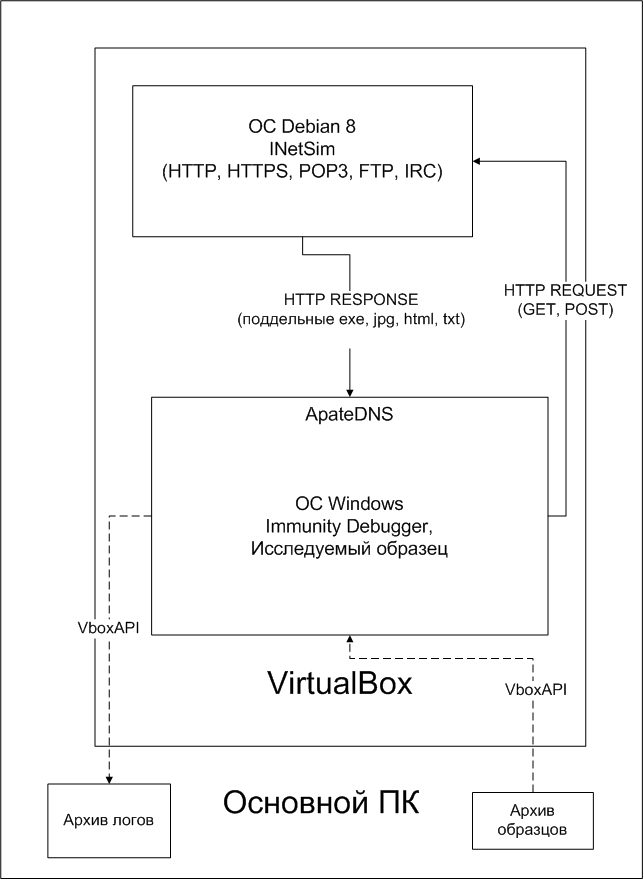
\includegraphics[width=\linewidth] {img/vmcycle.png}
	\caption {Пути взаимодействия компонентов системы сбора логов}
	\label {fig:vmcycle}
\end {figure}

\subsection {Предварительная конфигурация агента}
\subsubsection {Настройка окружения}
Здесь большинство действий было выполнено однократно, после чего был создан снапшот состояния с настроенным окружением, готового к запуску. Установлен отладчик Immunity Debugger, изменены его настройки, установлен Python 2.7.1, необходимый для работы отладчика, ApateDNS (утилита, позволяющая перенаправлять все DNS запросы на указанный IP адрес), .Net Framework 4.0, 4.5 (некоторые образцы построены с его использованием и не работают без него), выключен файрвол Windows и служба контроля учётных записей (User account control).
Далее на этом шаге просто происходит возврат в "чистое состояние" исследуемого агента и виртуальной машины с INetSim.
\subsubsection {Маскировка виртуальной среды}
Для маскировки исполнения в виртуальной среде были применены следующие модификации виртуальной машины:
\begin {itemize}
	\item Добавлена информация из DMI (Desktop Management Interface)

	DMI позволяет программному обеспечению получать информацию из BIOS, об оборудовании и материнской плате (скопирована с основного ПК с использованием утилиты dmidecode).
	\item Добавлена таблица ACPI (Advanced Configuration and Power Interface)

	ACPI реализует интерфейс для управления питанием и конфигурации материнской платы и устройств. Для этого в оперативной памяти размещается несколько таблиц, содержащих методы управления ими и их описание. При помощи утилиты acpidump с основного ПК была скопирована такая таблица и подключена к виртуальной машине.
	\item Сгенерирован случайный MAC сетевой карты

	По умолчанию присваиваемые MAC адреса относятся к диапазону, начинающемуся с 08-00-27 и могут быть таким образом обнаружены. Взят случайный адрес из диапазона Intel.
	\item Изменена информация об HDD
	\item Изменена информация о CD-приводе
	\item Модифицированы разделы реестра

	Изменены разделы реестра SystemBiosDate, VideoBiosVersion и др., имеющие значение по умолчанию при создании виртуальной машины, позволяющие идентифицировать её как экземпляр VirtualBox.
\end {itemize}
Данный функционал реализуется в рамках vbox/tools/HideVBox/camouflage.py

\subsection {Загрузка образца}
Используя vboxapi, реализован скрипт, скачивающий с основного ПК образец и скрипты, управляющие сбором логов.
\subsection {Запуск отслеживающих инструментов и исполнение образца}
Поскольку снапшот восстанавливаются из готового состояния, ApateDNS уже запущена и настроена на сервер INetSim.

Образец исполняется в отладчике, после чего специальный скрипт собирает информацию о присутствующих в таблице импортов исполняемого файла функций и устанавливает на них точки останова. Тот же скрипт регистрирует хук, в котором описаны необходимые для получения параметры в случае вызова таковых функций.
В случае вызова функции, отладчик логирует всё в файл. Образец исполняется в течение 2 мин.
\subsection {Получение логов}
По истечении указанного промежутка времени скрипт через vboxapi забирает собранные логи о деятельности образца и выключает обе виртуальные машины. После этого происходит выборка из архива следующего образца и запуск следующей итерации цикла для его исследования.



 
